\documentclass{article}

% content/resources/templates/preamble.tex
\usepackage[margin=0.6in]{geometry}
\author{Milav Dabgar}
\usepackage{amsmath,amssymb,amsthm}
\usepackage{booktabs}
\usepackage{multirow}
\usepackage{xcolor}
\usepackage{tcolorbox}
\tcbuselibrary{breakable,skins}
\usepackage[colorlinks=true,linkcolor=blue]{hyperref}
\usepackage{titlesec}
\usepackage{enumitem}
\usepackage{tikz}
\usepackage{pgfplots}
\usepackage{circuitikz}
\usepackage[version=4]{mhchem}
\usepackage{longtable}
\usepackage{array}
\usepackage{float}
\usepackage{caption}
\usepackage{listings}

\lstset{
  basicstyle=\small\ttfamily,
  breaklines=true,
  breakatwhitespace=false,
  postbreak=\mbox{\textcolor{red}{$\hookrightarrow$}\space},
  float=false,
  numbers=left,
  numberstyle=\tiny\color{gray},
  numbersep=10pt,
  xleftmargin=2em,
  keywordstyle=\color{blue},
  commentstyle=\color{green!60!black},
  stringstyle=\color{purple},
  backgroundcolor=\color{gray!5},
  showstringspaces=false,
  tabsize=2,
  captionpos=b,
  keepspaces=true,
  columns=flexible
}

\pgfplotsset{compat=1.18}
\usetikzlibrary{shapes,arrows,positioning,calc,patterns,decorations.pathmorphing,decorations.markings,arrows.meta}

% Color scheme
\definecolor{headcolor}{RGB}{0,102,204}
\definecolor{keycolor}{RGB}{220,20,60}
\definecolor{solutioncolor}{RGB}{34,139,34}
\definecolor{mnemoniccolor}{RGB}{148,0,211}
\definecolor{codecolor}{RGB}{0,0,100}

% Spacing
\setlength{\parskip}{3pt}
\setlist[itemize]{nosep}
\setlist[enumerate]{nosep}

% Title formatting
\titleformat{\section}{\Large\bfseries\color{headcolor}}{\thesection}{1em}{}
\titleformat{\subsection}{\large\bfseries\color{headcolor}}{\thesubsection}{1em}{}

% Pandoc tightlist compatibility
\providecommand{\tightlist}{%
  \setlength{\itemsep}{0pt}\setlength{\parskip}{0pt}}

% Pandoc longtable compatibility
\newcounter{none}
\def\thenone{}


% content/resources/templates/english-boxes.tex

% Custom environments
\newtcolorbox{solutionbox}{
 breakable,
 enhanced,
 colback=solutioncolor!5!white,
 colframe=solutioncolor!75!black,
 fonttitle=\bfseries,
 title=Solution
}

\newtcolorbox{solutionboxnobreak}{
 colback=solutioncolor!5!white,
 colframe=solutioncolor!75!black,
 fonttitle=\bfseries,
 title=Solution
}

\newtcolorbox{keyformula}{
 breakable,
 enhanced,
 colback=keycolor!5!white,
 colframe=keycolor!75!black,
 fonttitle=\bfseries,
 title=Key Formula
}

\newtcolorbox{mnemonicboxenv}{
 breakable,
 enhanced,
 colback=mnemoniccolor!5!white,
 colframe=mnemoniccolor!75!black,
 fonttitle=\bfseries,
 title=Mnemonic
}

\newcommand{\mnemonicbox}[1]{%
  \begin{mnemonicboxenv}
    #1
  \end{mnemonicboxenv}
}


% Custom commands for GTU solutions
% This file defines semantic commands for consistent formatting

% Question command with automatic formatting
\newcommand{\question}[2]{%
  \section*{Question #1}%
  \textbf{#2}%
}

% OR question variant
\newcommand{\questionor}[2]{%
  \section*{Question #1 OR}%
  \textbf{#2}%
}

% Proper table environment with caption
\newenvironment{answertable}[1]{%
  \begin{table}[htbp]
  \centering
  \caption{#1}
}{%
  \end{table}
}

% Proper figure environment for diagrams
\newenvironment{answerdiagram}[1]{%
  \begin{figure}[htbp]
  \centering
  \caption{#1}
}{%
  \end{figure}
}

% Semantic markup for key terms
\newcommand{\keyword}[1]{\textbf{#1}}
\newcommand{\code}[1]{\texttt{#1}}
\newcommand{\classname}[1]{\texttt{#1}}
\newcommand{\methodname}[1]{\texttt{#1}}

% Proper quotation marks
\newcommand{\mnemonic}[1]{``#1''}


\title{Industrial Electronics (4331103) - Summer 2024 Solution}
\date{June 12, 2024}

\begin{document}
\maketitle

\questionmarks{1(a)}{3}{Explain two transistor analogies of SCR.}

\begin{solutionbox}
SCR can be represented as a two-transistor model with interconnected PNP and NPN transistors.

\begin{center}
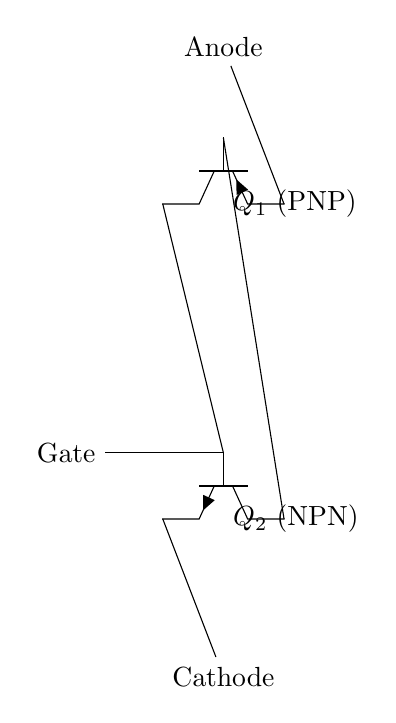
\begin{tikzpicture}[gtu block/.style={draw, rectangle, minimum width=2cm, minimum height=1cm, align=center}]
    % Transistors representation
    \node (anode) at (0,4) {Anode};
    \node (cathode) at (0,-4) {Cathode};
    
    % PNP Transistor Q1
    \draw (0,2) node[pnp, rotate=-90] (Q1) {};
    \node[right] at (Q1) {$Q_1$ (PNP)};
    
    % NPN Transistor Q2
    \draw (0,-2) node[npn, rotate=-90] (Q2) {};
    \node[right] at (Q2) {$Q_2$ (NPN)};
    
    % Connections
    \draw (anode) -- (Q1.E);
    \draw (Q1.C) -- (Q2.B);
    \draw (Q2.C) -- (Q1.B); % Feedback loop
    \draw (Q2.E) -- (cathode);
    
    % Gate
    \draw (Q2.B) -- ++(-1.5,0) node[left] {Gate};

\end{tikzpicture}
\captionof{figure}{Two Transistor Analogy of SCR}
\end{center}

\begin{itemize}
    \item \keyword{Regenerative action}: When gate current triggers NPN, it causes PNP to conduct, creating self-sustaining current
    \item \keyword{Latching mechanism}: Once both transistors are ON, gate loses control as feedback path maintains conduction
\end{itemize}
\end{solutionbox}
\mnemonicbox{Push-Pull Network Triggers Sustained Conduction}

\questionmarks{1(b)}{4}{Explain working and characteristic of IGBT.}

\begin{solutionbox}
IGBT (Insulated Gate Bipolar Transistor) combines MOSFET input characteristics with BJT output capabilities.

\begin{center}
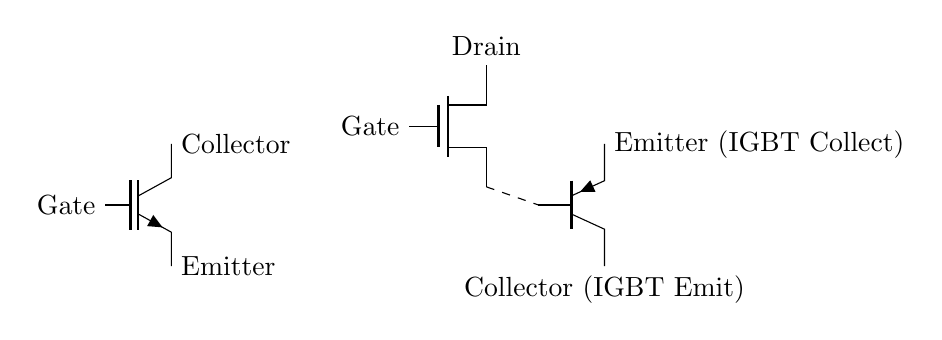
\begin{tikzpicture}
    % IGBT Symbol
    \draw (0,0) node[nigbt] (igbt) {};
    \node[right] at (igbt.C) {Collector};
    \node[right] at (igbt.E) {Emitter};
    \node[left] at (igbt.G) {Gate};
    
    % Equivalent Circuit Representation
    \draw (4, 1) node[nmos] (mos) {};
    \draw (5.5, 0) node[pnp] (bjt) {};
    
    \node[above] at (mos.D) {Drain};
    \node[left] at (mos.G) {Gate};
    \node[right] at (bjt.E) {Emitter (IGBT Collect)};
    \node[below] at (bjt.C) {Collector (IGBT Emit)};
    
    % Connections for equivalent circuit concept
    % Simplified conceptual link
    \draw[dashed] (mos.S) -- (bjt.B); 
\end{tikzpicture}
\captionof{figure}{IGBT Symbol and Structure}
\end{center}

\begin{center}
\begin{tabulary}{\linewidth}{|L|L|}
\hline \textbf{Feature} & \textbf{Characteristic} \\ \hline
Switching & Fast turn-on, moderate turn-off \\
Control & Voltage-controlled like MOSFET \\
Conduction & Low forward voltage drop like BJT \\
Applications & High voltage, medium frequency switching \\
\hline
\end{tabulary}
\captionof{table}{IGBT Characteristics}
\end{center}

\begin{itemize}
    \item \keyword{Input advantage}: Voltage-controlled gate with high impedance requires minimal drive power
    \item \keyword{Output advantage}: Low on-state voltage drop even at high current densities
\end{itemize}
\end{solutionbox}
\mnemonicbox{MOSFET Input, BJT Output, Makes Perfect Power Switch}

\questionmarks{1(c)}{7}{Explain construction, working and characteristic of DIAC.}

\begin{solutionbox}
DIAC (DIode for Alternating Current) is a bidirectional triggering device used in thyristor control circuits.

\begin{center}
\begin{tikzpicture}
    % Construction
    \draw (0,0) rectangle (4,2);
    \draw (0,1.5) -- (4,1.5);
    \draw (0,0.5) -- (4,0.5);
    \node at (2, 1.75) {N2 (Terminal B)};
    \node at (2, 1) {P2 - N1 - P1};
    \node at (2, 0.25) {N1 (Terminal A)};
    
    % Symbol
    \draw (6,1) to[diac] (8,1);
    \node[left] at (6,1) {MT1};
    \node[right] at (8,1) {MT2};
\end{tikzpicture}
\captionof{figure}{DIAC Construction and Symbol}
\end{center}

\begin{center}
\begin{tikzpicture}
    % V-I Curve
    \draw[->] (-3,0) -- (3,0) node[right] {$V$};
    \draw[->] (0,-3) -- (0,3) node[above] {$I$};
    
    \draw[blue, thick] (0,0) -- (1,0.1) -- (2, 2) -- (1.5, 2.5);
    \draw[blue, thick] (0,0) -- (-1,-0.1) -- (-2, -2) -- (-1.5, -2.5);
    
    \node[right] at (2,2) {$V_{BO}$};
    \node[left] at (-2,-2) {$-V_{BO}$};
\end{tikzpicture}
\captionof{figure}{DIAC V-I Characteristics}
\end{center}

\begin{center}
\begin{tabulary}{\linewidth}{|L|L|}
\hline \textbf{Feature} & \textbf{Description} \\ \hline
Structure & Five-layer P-N-P-N with no gate terminal \\
Operation & Blocks current until break-over voltage is reached \\
Breakover & Typically 30-40V in either direction \\
Symmetry & Identical response in both directions \\
Application & Trigger device for TRIACs in AC circuits \\
\hline
\end{tabulary}
\captionof{table}{DIAC Features}
\end{center}

\begin{itemize}
    \item \keyword{Blocking state}: Below breakover voltage, high resistance prevents current flow
    \item \keyword{Conducting state}: Above breakover voltage, negative resistance region enables sudden conduction
    \item \keyword{Bidirectional}: Functions identically for positive and negative voltages
\end{itemize}
\end{solutionbox}
\mnemonicbox{Break Voltage Both Ways, Then Current Flows}

\questionmarks{1(c) OR}{7}{Explain construction and working of Opto-Isolator and Opto-SCR}

\begin{solutionbox}
Opto-devices use light to transfer signals while maintaining electrical isolation between circuits.

\begin{center}
\begin{tikzpicture}
    % Opto-Isolator
    \draw[dashed] (-1,-1) rectangle (3,2);
    \node at (1,2.3) {Opto-Isolator};
    \draw (0,0.5) node[led, rotate=90] (led) {};
    \draw (led.anode) -- (0, 1.5) node[above] {In+};
    \draw (led.cathode) -- (0, -0.5) node[below] {In-};
    
    \draw (2,0.5) node[npn, photo] (photo) {};
    \draw (photo.C) -- (2,1.5) node[above] {VCC};
    \draw (photo.E) -- (2,-0.5) node[below] {Out};
    
    \draw[->, wave] (0.5, 0.5) -- (1.5, 0.5);
\end{tikzpicture}
\captionof{figure}{Opto-Isolator}
\end{center}

\begin{center}
\begin{tikzpicture}
    % Opto-SCR
    \draw[dashed] (-1,-1) rectangle (3,2);
    \node at (1,2.3) {Opto-SCR};
    \draw (0,0.5) node[led, rotate=90] (led) {};
    \draw (led.anode) -- (0, 1.5) node[above] {In+};
    \draw (led.cathode) -- (0, -0.5) node[below] {In-};
    
    \draw (2,0.5) node[thyristor] (scr) {};
    \draw (scr.A) -- (2,1.5) node[above] {A};
    \draw (scr.K) -- (2,-0.5) node[below] {K};
    
    \draw[->, wave] (0.5, 0.5) -- (1.5, 0.5);
\end{tikzpicture}
\captionof{figure}{Opto-SCR}
\end{center}

\begin{center}
\begin{tabulary}{\linewidth}{|L|L|L|}
\hline \textbf{Feature} & \textbf{Opto-Isolator} & \textbf{Opto-SCR} \\ \hline
Input & LED & LED \\
Output device & Phototransistor/photodiode & Light-sensitive SCR \\
Isolation & 2-5 kV & 2-5 kV \\
Current handling & Low-medium (100mA) & High (several amps) \\
Applications & Digital signal isolation & Power control, AC switching \\
\hline
\end{tabulary}
\captionof{table}{Comparison of Opto-Devices}
\end{center}

\begin{itemize}
    \item \keyword{Electrical isolation}: Complete electrical separation provides noise immunity and safety
    \item \keyword{Signal transfer}: Light coupling eliminates ground loops and voltage level issues
    \item \keyword{Triggering}: Light replaces gate current for SCR activation in Opto-SCR
\end{itemize}
\end{solutionbox}
\mnemonicbox{Light Jumps Gaps While Electricity Stays Home}

\questionmarks{2(a)}{3}{Draw symbol and give application of 1) UJT 2) SCS 3) MCT.}

\begin{solutionbox}
\begin{center}
\begin{tabulary}{\linewidth}{|C|C|L|}
\hline \textbf{Device} & \textbf{Symbol} & \textbf{Applications} \\ \hline
UJT & 
\begin{tikzpicture}[scale=0.5, baseline]
    \draw (0,0) node[ujt] {};
\end{tikzpicture} & 
Relaxation oscillators, timing circuits, SCR triggering \\ \hline
SCS & 
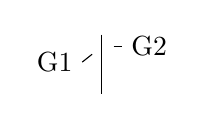
\begin{tikzpicture}[scale=0.5, baseline]
    \draw (0,0) -- (0,-0.5) node[thyristor] (T) {} -- (0,-1.5);
    \draw (T.west) -- (-0.5, -0.7) node[left] {G1};
    \draw (0.3, -0.3) -- (0.5, -0.3) node[right] {G2}; 
\end{tikzpicture} & 
Low power switching, level detection, pulse generation \\ \hline
MCT & 
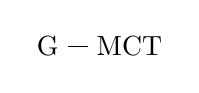
\begin{tikzpicture}[scale=0.5, baseline]
    % Simple MCT representation: Thyristor with MOS gate structure
    \draw (0,0) node[thyristor] (T) {};
    \draw (T.west) -- ++(-0.5,0) node[left] {G};
    \node at (0.8,0) {MCT};
\end{tikzpicture} & 
High power switching, motor control, inverters \\ \hline
\end{tabulary}
\captionof{table}{Power Devices Symbols and Applications}
\end{center}
\end{solutionbox}
\mnemonicbox{Unique timing, Controlled switching, Master power}

\questionmarks{2(b)}{4}{Explain importance of gate protection for SCR.}

\begin{solutionbox}
Gate protection circuits safeguard SCR against spurious triggering and voltage spikes.

\begin{center}
\begin{tikzpicture}
    \draw (0,0) node[thyristor] (S) {};
    \draw (S.G) -- (-2, -0.7); % Gate line
    
    % Protection components
    \draw (-1, -0.7) to[R, l=$R_g$] (-1, -2) node[ground]{}; % Gate resistor
    \draw (-1.5, -0.7) to[D, l=D] (-1.5, -2) node[ground]{}; % Protecting Diode
    
    \node at (0, 1) {Anode};
    \node at (0, -2) {Cathode};
\end{tikzpicture}
\captionof{figure}{Gate Protection Circuit}
\end{center}

\begin{center}
\begin{tabulary}{\linewidth}{|L|L|L|}
\hline \textbf{Problem} & \textbf{Protection Method} & \textbf{Purpose} \\ \hline
Reverse voltage & Diode across gate & Prevents gate-cathode junction damage \\
Noise & RC filter & Blocks high-frequency transients \\
dV/dt triggering & RC snubber & Controls rate of voltage rise \\
False triggering & Gate resistor & Limits gate current and avoids noise triggering \\
\hline
\end{tabulary}
\captionof{table}{Gate Protection Methods}
\end{center}

\begin{itemize}
    \item \keyword{Junction protection}: Prevents reverse voltage damage to gate-cathode junction
    \item \keyword{Noise immunity}: Filters out electrical noise that could cause unwanted triggering
\end{itemize}
\end{solutionbox}
\mnemonicbox{Guard the Gate to Prevent Problems}

\questionmarks{2(c)}{7}{List out various methods of triggering SCR and explain any three of them.}

\begin{solutionbox}
SCR triggering methods convert the device from blocking to conducting state through gate activation.

\begin{center}
\begin{tabulary}{\linewidth}{|L|L|L|}
\hline \textbf{Method} & \textbf{Principle} & \textbf{Applications} \\ \hline
Gate triggering & Direct current to gate & Most common method \\
Thermal triggering & Temperature increase & Thermal protection \\
Light triggering & Photons on junction & Remote activation \\
dV/dt triggering & Fast voltage rise & Often undesirable triggering \\
Voltage triggering & Exceeding breakover voltage & Protection circuits \\
RF triggering & Radio frequency signals & Wireless control \\
\hline
\end{tabulary}
\captionof{table}{Triggering Methods Overview}
\end{center}

\textbf{1. Gate Current Triggering:}
\begin{center}
\begin{tikzpicture}
    \draw (0,0) node[thyristor] (S) {};
    \draw (S.G) -- (-2, -0.7) to[battery] (-2, -2) -- (S.K);
    \node at (-1.5, -1) {$I_g$};
\end{tikzpicture}
\end{center}
\begin{itemize}
    \item \keyword{Direct control}: Small gate current initiates large anode current flow
    \item \keyword{Current range}: 10-100mA typically required depending on SCR rating
\end{itemize}

\textbf{2. Light Triggering (LASCR):}
\begin{center}
\begin{tikzpicture}
    \draw (0,0) node[thyristor] (S) {};
    \draw[->, wave] (-1.5, 0) -- (-0.5, 0);
    \node at (-2, 0) {Light};
\end{tikzpicture}
\end{center}
\begin{itemize}
    \item \keyword{Optical control}: Photons generate carriers at junction
    \item \keyword{Isolation}: Provides electrical isolation between control and power circuit
\end{itemize}

\textbf{3. dV/dt Triggering:}
\begin{center}
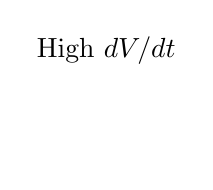
\begin{tikzpicture}
    \draw (0,0) node[thyristor] (S) {};
    \draw (0,1) node[above] {High $dV/dt$};
\end{tikzpicture}
\end{center}
\begin{itemize}
    \item \keyword{Rate sensitivity}: Rapid voltage rise causes junction capacitance charging
    \item \keyword{Prevention}: Snubber circuits (RC networks) control voltage rise rate
\end{itemize}
\end{solutionbox}
\mnemonicbox{Gates, Light, and Voltage Changes Turn SCRs On}

\questionmarks{2(a) OR}{3}{Explain working of solid state relay using opto-SCR.}

\begin{solutionbox}
Solid state relays (SSRs) use opto-SCR for contactless switching with electrical isolation.

\begin{center}
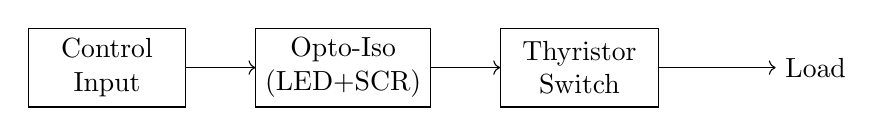
\begin{tikzpicture}[gtu block/.style={draw, rectangle, minimum width=2cm, minimum height=1cm, align=center}, node distance=3cm]
    \node[gtu block] (in) {Control \\ Input};
    \node[gtu block, right of=in] (iso) {Opto-Iso \\ (LED+SCR)};
    \node[gtu block, right of=iso] (sw) {Thyristor \\ Switch};
    \node[right of=sw] (load) {Load};
    
    \draw[->] (in) -- (iso);
    \draw[->] (iso) -- (sw);
    \draw[->] (sw) -- (load);
\end{tikzpicture}
\captionof{figure}{SSR Block Diagram}
\end{center}

\begin{center}
\begin{tabulary}{\linewidth}{|L|L|L|}
\hline \textbf{Stage} & \textbf{Function} & \textbf{Benefit} \\ \hline
Input stage & Drives LED using control signal & Low power control \\
Isolation & Light bridges electrical gap & Safety and noise immunity \\
Triggering & Light activates SCR & No mechanical contacts \\
Switching & Thyristors conduct load current & No arcing or contact wear \\
\hline
\end{tabulary}
\captionof{table}{SSR Operation}
\end{center}

\begin{itemize}
    \item \keyword{Silent operation}: No mechanical noise during switching
    \item \keyword{Long life}: No contact degradation as in electromechanical relays
\end{itemize}
\end{solutionbox}
\mnemonicbox{Light Links Logic to Load}

\questionmarks{2(b) OR}{4}{Define snubber circuit and explain importance of snubber circuit.}

\begin{solutionbox}
A snubber circuit is a protective network that suppresses voltage and current transients in switching devices.

\begin{center}
\begin{tikzpicture}
    \draw (0,0) node[thyristor] (S) {};
    \draw (S.north) -- (0, 2);
    \draw (S.south) -- (0, -2);
    
    % Snubber R-C
    \draw (0,1.5) -- (2,1.5) to[R, l=$R_s$] (2,0) to[C, l=$C_s$] (2,-1.5) -- (0,-1.5);
\end{tikzpicture}
\captionof{figure}{RC Snubber Circuit}
\end{center}

\begin{center}
\begin{tabulary}{\linewidth}{|L|L|L|}
\hline \textbf{Function} & \textbf{Benefit} & \textbf{Implementation} \\ \hline
dV/dt suppression & Prevents false triggering & RC circuit across SCR \\
Voltage spike reduction & Protects from overvoltage & Capacitor absorbs energy \\
Oscillation damping & Reduces EMI & Resistor provides damping \\
Turn-off assistance & Improves commutation & Diverts current during turn-off \\
\hline
\end{tabulary}
\captionof{table}{Snubber Importance}
\end{center}

\begin{itemize}
    \item \keyword{Circuit protection}: Extends thyristor life by limiting stress on the device
    \item \keyword{Noise reduction}: Minimizes electromagnetic interference in surrounding circuits
\end{itemize}
\end{solutionbox}
\mnemonicbox{Suppress Noise Upsetting Balanced Behaviors Easily Restored}

\questionmarks{2(c) OR}{7}{List various commutation methods of SCR and explain any two of them}

\begin{solutionbox}
Commutation is the process of turning OFF an SCR by reducing its anode current below holding value.

\begin{center}
\begin{tabulary}{\linewidth}{|L|L|L|}
\hline \textbf{Method} & \textbf{Principle} & \textbf{Applications} \\ \hline
Natural & AC zero crossing & AC power control \\
Forced & External circuit & DC applications \\
Class A & LC resonance & Inverters \\
Class B & Auxiliary SCR & DC choppers \\
Class C & LC with load & Variable frequency \\
Class D & Auxiliary source & Motor control \\
Class E & External pulse & Electronic circuits \\
\hline
\end{tabulary}
\captionof{table}{Commutation Methods}
\end{center}

\textbf{1. Natural Commutation:}
\begin{center}
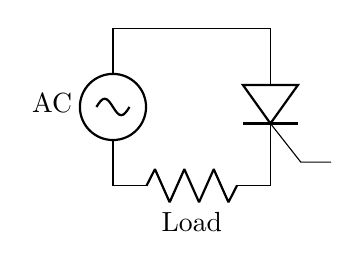
\begin{tikzpicture}
    \draw (0,0) to[sV, l=AC] (0,2) -- (2,2) to[thyristor] (2,0) to[R, l=Load] (0,0);
\end{tikzpicture}
\captionof{figure}{Natural Commutation}
\end{center}
\begin{itemize}
    \item \keyword{Zero crossing}: SCR turns off when AC crosses zero and anode current falls below holding
    \item \keyword{Simplicity}: No additional components required for commutation
    \item \keyword{Limitation}: Works only in AC circuits at fixed frequency
\end{itemize}

\textbf{2. Forced Commutation (Class B):}
\begin{center}
\begin{tikzpicture}
    \draw (0,3) -- (2,3) node[above] {Vdc} -- (4,3);
    \draw (2,3) to[thyristor, l=SCR1] (2,0);
    \draw (4,3) to[C] (4,1.5) -- (2,1.5); % Capacitor coupling
    \draw (4,3) -- (6,3) to[thyristor, l=SCR2] (6,0);
    \draw (2,0) to[R, l=Load] (2,-2) node[ground]{};
    \draw (6,0) -- (6,-2) node[ground]{};
\end{tikzpicture}
\captionof{figure}{Class B Commutation}
\end{center}
\begin{itemize}
    \item \keyword{Auxiliary SCR}: Second SCR (SCR2) discharges capacitor to reverse bias main SCR
    \item \keyword{Timing control}: Precise control over when SCR turns off
    \item \keyword{Application}: Used in DC circuits where natural commutation isn't possible
\end{itemize}
\end{solutionbox}
\mnemonicbox{Nature Follows Current, Forced Creates Current Collapse}

\questionmarks{3(a)}{3}{Explain advantages of polyphase rectifier over single phase rectifier.}

\begin{solutionbox}
Polyphase rectifiers offer significant improvements over single-phase designs in power applications.

\begin{center}
\begin{tabulary}{\linewidth}{|L|L|L|}
\hline \textbf{Parameter} & \textbf{Single Phase} & \textbf{Polyphase} \\ \hline
Ripple factor & Higher (0.482 for FW) & Lower (0.042 for 3-phase) \\
Form factor & Higher & Lower \\
Efficiency & Lower & Higher (better transformer utilization) \\
Power rating & Limited & Higher power handling \\
Harmonic content & More & Less (smoother DC) \\
\hline
\end{tabulary}
\captionof{table}{Single Phase vs Polyphase Rectifiers}
\end{center}

\begin{itemize}
    \item \keyword{Output smoothness}: Significantly less ripple requiring smaller filtering components
    \item \keyword{Transformer utilization}: Better utilization factor (0.955 vs 0.812) reduces transformer size
\end{itemize}
\end{solutionbox}
\mnemonicbox{More Phases Mean Smoother Power}

\questionmarks{3(b)}{4}{Write short note on UPS.}

\begin{solutionbox}
UPS (Uninterruptible Power Supply) provides continuous power during main supply failure.

\begin{center}
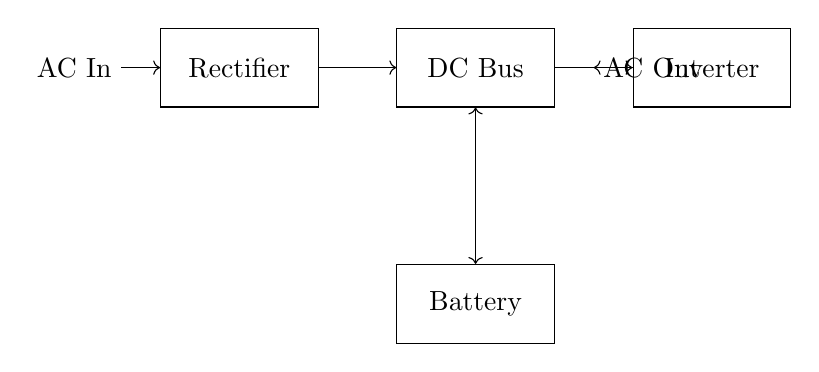
\begin{tikzpicture}[gtu block/.style={draw, rectangle, minimum width=2cm, minimum height=1cm, align=center}, node distance=3cm]
    \node[gtu block] (rect) {Rectifier};
    \node[gtu block, right of=rect] (dc) {DC Bus};
    \node[gtu block, right of=dc] (inv) {Inverter};
    \node[gtu block, below of=dc] (batt) {Battery};
    
    \draw[->] (-1.5, 0) node[left]{AC In} -- (rect);
    \draw[->] (rect) -- (dc);
    \draw[->] (dc) -- (inv);
    \draw[->] (inv) -- (4.5, 0) node[right]{AC Out};
    \draw[<->] (dc) -- (batt);
\end{tikzpicture}
\captionof{figure}{Basic UPS Block Diagram}
\end{center}

\begin{center}
\begin{tabulary}{\linewidth}{|L|L|L|}
\hline \textbf{Type} & \textbf{Operation} & \textbf{Applications} \\ \hline
Online & Always through battery/inverter & Critical systems, medical \\
Offline & Switches to battery on failure & Personal computers, small offices \\
Line-interactive & Voltage regulation + backup & Servers, network equipment \\
\hline
\end{tabulary}
\captionof{table}{UPS Types}
\end{center}

\begin{itemize}
    \item \keyword{Backup time}: Typically 5-30 minutes depending on battery capacity
    \item \keyword{Protection}: Surge protection, voltage regulation, and frequency stabilization
\end{itemize}
\end{solutionbox}
\mnemonicbox{Power Constantly Protected Under Switch}

\questionmarks{3(c)}{7}{Give function of Inverter and explain basic principle of Inverter also explain series inverter with neat diagram and waveform.}

\begin{solutionbox}
Inverters convert DC power to AC power by switching DC through a transformer or directly to create alternating waveforms.

\begin{center}
\begin{tabulary}{\linewidth}{|L|L|}
\hline \textbf{Function} & \textbf{Description} \\ \hline
DC to AC conversion & Transforms steady DC to alternating AC \\
Frequency control & Generates variable frequency output \\
Voltage regulation & Maintains stable output despite load variations \\
Wave shaping & Produces sine, square, or modified sine waves \\
\hline
\end{tabulary}
\captionof{table}{Inverter Functions}
\end{center}

\textbf{Series Inverter Circuit:}
\begin{center}
\begin{tikzpicture}
    % Series Inverter
    \draw (0,4) -- (4,4) node[right]{+Vdc};
    \draw (0,0) -- (4,0) node[right]{GND};
    
    \draw (2,4) -- (2,3) to[L, l=$L$] (2,2) to[C, l=$C$] (2,1) -- (2,0.5);
    \draw (2,0.5) node[thyristor] (T) {};
    \draw (T.south) -- (2, -1) to[R, l=Load] (2,-2) node[ground]{};
    
    % Simplified conceptual schematic for series resonant
    % Actually usually comprises two SCRs and L-C-R load. 
    % Let's draw a standard Series Inverter (Class A)
    % +VDC - SCR1 - L - C - Load - GND. (Half wave)
\end{tikzpicture}
\end{center}
\begin{itemize}
    \item \keyword{Oscillation}: Series LC circuit creates resonant oscillation when SCR triggers
    \item \keyword{Commutation}: SCR turns off naturally when current reverses through resonance
    \item \keyword{Frequency}: Determined by LC values: $f = 1/(2\pi\sqrt{LC})$
\end{itemize}
\end{solutionbox}
\mnemonicbox{Direct Current Switches To Alternating Current Through Resonant Circuit}

\questionmarks{3(a) OR}{3}{Explain basic principle of chopper.}

\begin{solutionbox}
A chopper is a DC-to-DC converter that switches DC input on/off to produce controllable average DC output.

\begin{center}
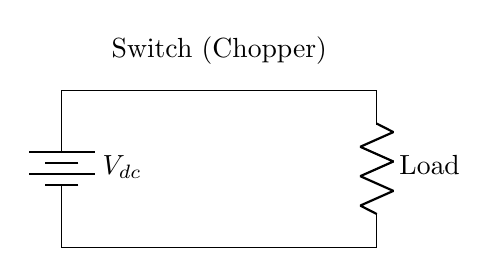
\begin{tikzpicture}
    \draw (0,2) to[battery, l=$V_{dc}$] (0,0);
    \draw (0,2) -- (2,2) node[switch] (S) {} -- (4,2);
    \draw (4,2) to[R, l=Load] (4,0) -- (0,0);
    \node at (2,2.5) {Switch (Chopper)};
\end{tikzpicture}
\captionof{figure}{Basic Chopper Circuit}
\end{center}

\begin{center}
\begin{tabulary}{\linewidth}{|L|L|L|}
\hline \textbf{Parameter} & \textbf{Relation} & \textbf{Control} \\ \hline
Output voltage & $V_o = V_{dc} \times (T_{on}/T)$ & Duty cycle adjustment \\
Duty cycle & $k = T_{on}/T$ & Controls output voltage \\
Frequency & $f = 1/T$ & Affects ripple \\
Voltage regulation & Varies with load & Feedback control adjusts duty cycle \\
\hline
\end{tabulary}
\captionof{table}{Chopper Principle}
\end{center}

\begin{itemize}
    \item \keyword{Switching action}: Rapidly turns ON/OFF to chop DC input
    \item \keyword{Pulse width modulation}: Controls voltage by varying ON-time ratio
\end{itemize}
\end{solutionbox}
\mnemonicbox{Chopping Creates Controllable DC}

\questionmarks{3(b) OR}{4}{Draw the block diagram of SMPS and explain function of each block.}

\begin{solutionbox}
SMPS (Switched Mode Power Supply) converts input power to regulated output using high-frequency switching.

\begin{center}
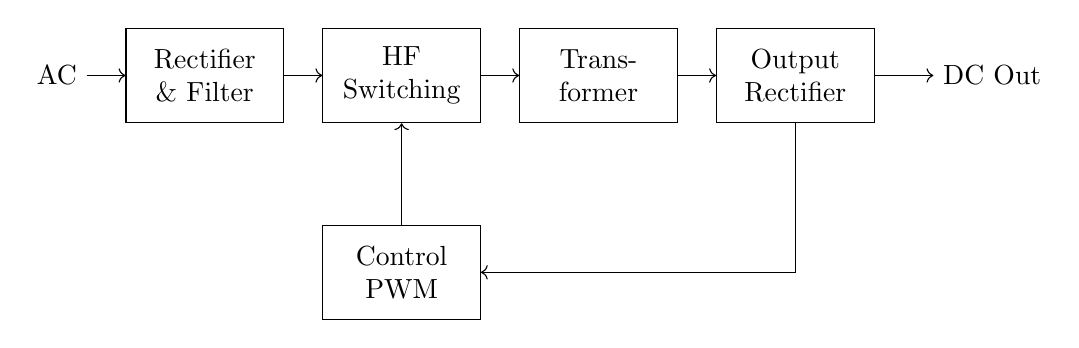
\begin{tikzpicture}[gtu block/.style={draw, rectangle, minimum width=2cm, minimum height=1.2cm, align=center}, node distance=2.5cm, auto]
    \node[gtu block] (rect) {Rectifier \\ \& Filter};
    \node[gtu block, right of=rect] (switch) {HF \\ Switching};
    \node[gtu block, right of=switch] (trans) {Trans- \\ former};
    \node[gtu block, right of=trans] (outrect) {Output \\ Rectifier};
    \node[right of=outrect] (load) {DC Out};
    
    \node[gtu block, below of=switch] (ctrl) {Control \\ PWM};
    
    \draw[->] (-1.5, 0) node[left]{AC} -- (rect);
    \draw[->] (rect) -- (switch);
    \draw[->] (switch) -- (trans);
    \draw[->] (trans) -- (outrect);
    \draw[->] (outrect) -- (load);
    \draw[->] (outrect) |- (ctrl);
    \draw[->] (ctrl) -- (switch);
\end{tikzpicture}
\captionof{figure}{SMPS Block Diagram}
\end{center}

\begin{center}
\begin{tabulary}{\linewidth}{|L|L|}
\hline \textbf{Block} & \textbf{Function} \\ \hline
EMI Filter & Suppresses noise from entering/leaving SMPS \\
Rectifier \& Filter & Converts AC to unregulated DC \\
Switching Circuit & Chops DC at high frequency (20-200kHz) \\
Transformer & Provides isolation and voltage transformation \\
Output Rectifier & Converts high-frequency AC back to DC \\
Output Filter & Smooths DC output and removes ripple \\
Feedback Control & Regulates output by adjusting duty cycle \\
\hline
\end{tabulary}
\captionof{table}{SMPS Block Functions}
\end{center}

\begin{itemize}
    \item \keyword{High efficiency}: 70-90\% vs 30-60\% for linear supplies
    \item \keyword{Small size}: High frequency allows smaller transformer and components
\end{itemize}
\end{solutionbox}
\mnemonicbox{Filter, Rectify, Switch Through Transformer, Rectify, Filter}

\questionmarks{3(c) OR}{7}{Explain 1 phase half wave rectifier with waveform also explain 3 phase full wave rectifier with waveform.}

\begin{solutionbox}
Rectifiers convert AC to DC by allowing current flow in one direction while blocking reverse flow.

\textbf{1-Phase Half Wave Rectifier:}
\begin{center}
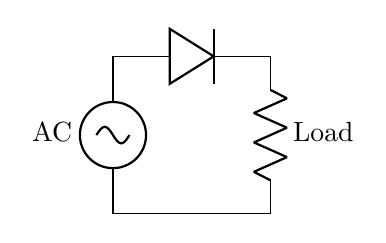
\begin{tikzpicture}
    \draw (0,0) to[sV, l=AC] (0,2) to[D] (2,2) to[R, l=Load] (2,0) -- (0,0);
\end{tikzpicture}
\end{center}

\textbf{3-Phase Full Wave Rectifier:}
\begin{center}
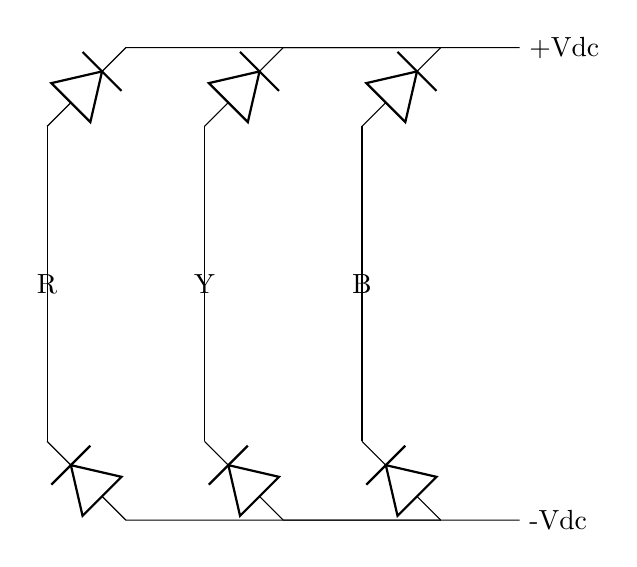
\begin{tikzpicture}
    % 3 Phase bridge
    \draw (0,0) -- (0,4);
    \draw (2,0) -- (2,4);
    \draw (4,0) -- (4,4);
    
    % Diodes on top
    \draw (0,4) to[D] (1,5) -- (5,5);
    \draw (2,4) to[D] (3,5) -- (5,5);
    \draw (4,4) to[D] (5,5) -- (6,5) node[right]{+Vdc};
    
    % Diodes on bottom
    \draw (0,0) to[D, invert] (1,-1) -- (5,-1);
    \draw (2,0) to[D, invert] (3,-1) -- (5,-1);
    \draw (4,0) to[D, invert] (5,-1) -- (6,-1) node[right]{-Vdc};
    
    % Inputs
    \node at (0,2) {R};
    \node at (2,2) {Y};
    \node at (4,2) {B};
\end{tikzpicture}
\end{center}

\begin{center}
\begin{tabulary}{\linewidth}{|L|L|L|}
\hline \textbf{Parameter} & \textbf{1-Phase Half Wave} & \textbf{3-Phase Full Wave} \\ \hline
Ripple factor & 1.21 & 0.042 \\
Rectification efficiency & 40.6\% & 95.5\% \\
TUF & 0.287 & 0.955 \\
Peak inverse voltage & $V_m$ & $2.09V_m$ \\
Form factor & 1.57 & 1.0007 \\
\hline
\end{tabulary}
\captionof{table}{Rectifier Comparison}
\end{center}

\begin{itemize}
    \item \keyword{1-Phase Half Wave}: Simplest design but with high ripple and poor efficiency
    \item \keyword{3-Phase Full Wave}: Much smoother output with 6 pulses per cycle
\end{itemize}
\end{solutionbox}
\mnemonicbox{Half Passes Only Peaks, Three Phases Fill Valleys}

\questionmarks{4(a)}{3}{Describe working of solar photovoltaic based power generation with block diagram.}

\begin{solutionbox}
Solar PV power generation converts sunlight directly into electricity through photovoltaic effect.

\begin{center}
\begin{tikzpicture}[gtu block/.style={draw, rectangle, minimum width=2cm, minimum height=1cm, align=center}, node distance=2.5cm]
    \node[gtu block] (solar) {Solar \\ Array};
    \node[gtu block, right of=solar] (charge) {Charge \\ Controller};
    \node[gtu block, below of=charge] (batt) {Battery};
    \node[gtu block, right of=charge] (inv) {Inverter};
    \node[right of=inv] (ac) {AC Load};
    \node[above of=charge] (dc) {DC Load};
    
    \draw[->] (solar) -- (charge);
    \draw[<->] (charge) -- (batt);
    \draw[->] (charge) -- (inv);
    \draw[->] (inv) -- (ac);
    \draw[->] (charge) -- (dc);
\end{tikzpicture}
\captionof{figure}{Solar PV System}
\end{center}

\begin{center}
\begin{tabulary}{\linewidth}{|L|L|}
\hline \textbf{Component} & \textbf{Function} \\ \hline
Solar panels & Convert sunlight to DC electricity \\
Charge controller & Regulates charging, prevents overcharge \\
Battery bank & Stores energy for later use \\
Inverter & Converts DC to AC for household appliances \\
Distribution panel & Routes electricity to loads \\
\hline
\end{tabulary}
\captionof{table}{PV Components}
\end{center}

\begin{itemize}
    \item \keyword{Energy conversion}: Photons excite electrons in semiconductor material creating current
    \item \keyword{Scalability}: System size can be adjusted based on power requirements
\end{itemize}
\end{solutionbox}
\mnemonicbox{Sunlight Produces Voltage, Batteries Invert Loads}

\questionmarks{4(b)}{4}{Explain use of SCR as static switch.}

\begin{solutionbox}
SCR functions as a solid-state switch with no moving parts for reliable and fast switching.

\begin{center}
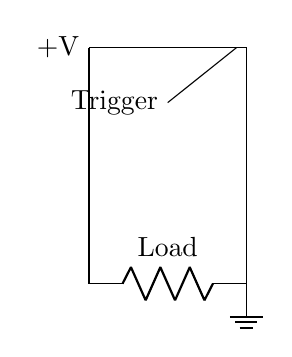
\begin{tikzpicture}
    \draw (0,3) -- (2,3) node[thyristor] (T) {} -- (2,0);
    \draw (0,3) node[left] {+V} -- (0,0) to[R, l=Load] (2,0) node[ground]{};
    \draw (T.west) -- (1, 2.3) node[left] {Trigger};
\end{tikzpicture}
\captionof{figure}{SCR Static Switch Concept}
\end{center}

\begin{center}
\begin{tabulary}{\linewidth}{|L|L|L|}
\hline \textbf{Application} & \textbf{Advantage} & \textbf{Implementation} \\ \hline
Power control & Precise control, no arcing & Phase angle control \\
Motor starting & Smooth acceleration & Gradual voltage increase \\
Circuit protection & Fast response & Current sensing trigger \\
Heating control & Energy efficient & Zero-crossing switching \\
\hline
\end{tabulary}
\captionof{table}{Static Switch Applications}
\end{center}

\begin{itemize}
    \item \keyword{Latching action}: Once triggered, continues to conduct until current falls below holding value
    \item \keyword{High reliability}: No mechanical wear due to absence of moving parts
\end{itemize}
\end{solutionbox}
\mnemonicbox{Semiconductor Switching Controls Running Loads}

\questionmarks{4(c)}{7}{Describe the working principle of Induction heating and dielectric heating also give comparison of Induction heating and dielectric heating.}

\begin{solutionbox}
Both heating methods use electromagnetic principles to generate heat without direct contact.

\begin{center}
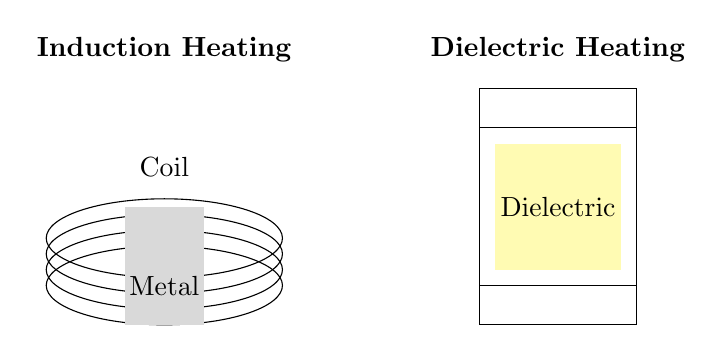
\begin{tikzpicture}
    % Induction
    \node at (0,3) {\textbf{Induction Heating}};
    \draw (0,0) ellipse (1.5 and 0.5);
    \foreach \y in {0.2, 0.4, 0.6} \draw (0,\y) ellipse (1.5 and 0.5);
    \node at (0,1.5) {Coil};
    \fill[gray!30] (-0.5, -0.5) rectangle (0.5, 1);
    \node at (0,0) {Metal};
    
    % Dielectric
    \node at (5,3) {\textbf{Dielectric Heating}};
    \draw (4,0) rectangle (6, 2);
    \fill[yellow!30] (4.2, 0.2) rectangle (5.8, 1.8);
    \node at (5,1) {Dielectric};
    \draw (4,2) -- (4,2.5) -- (6,2.5) -- (6,2); % Plate 1
    \draw (4,0) -- (4,-0.5) -- (6,-0.5) -- (6,0); % Plate 2
\end{tikzpicture}
\captionof{figure}{Heating Principles}
\end{center}

\begin{center}
\begin{tabulary}{\linewidth}{|L|L|L|}
\hline \textbf{Parameter} & \textbf{Induction Heating} & \textbf{Dielectric Heating} \\ \hline
Principle & Eddy currents and hysteresis & Molecular friction from oscillating field \\
Materials & Conductive metals & Non-conductive materials (plastics, wood) \\
Frequency & 1-100 kHz & 10-100 MHz \\
Penetration & Surface and shallow depth & Uniform through material \\
Efficiency & 80-90\% & 50-70\% \\
Applications & Metal hardening, melting, forging & Plastic welding, food processing, drying \\
\hline
\end{tabulary}
\captionof{table}{Heating Methods Comparison}
\end{center}

\begin{itemize}
    \item \keyword{Induction heating}: Works through electromagnetic induction creating eddy currents in conductive materials
    \item \keyword{Dielectric heating}: Causes rapid oscillation of polar molecules creating internal friction and heat
\end{itemize}
\end{solutionbox}
\mnemonicbox{Induction Makes Metals Hot, Dielectrics Heat Non-Metals}

\questionmarks{4(a) OR}{3}{Draw and explain the circuit diagram of photo electric relay using photo diode.}

\begin{solutionbox}
Photo-electric relay uses light detection to control switching operations automatically.

\begin{center}
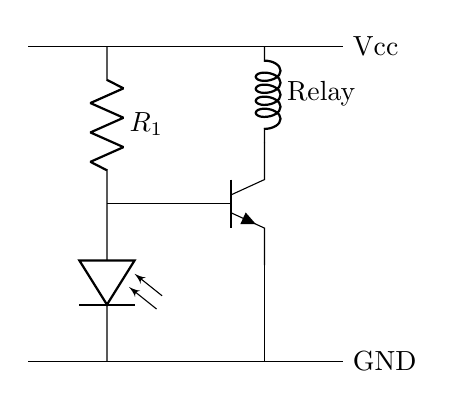
\begin{tikzpicture}
    % Photo Relay
    \draw (0,4) -- (4,4) node[right]{Vcc};
    \draw (0,0) -- (4,0) node[right]{GND};
    
    \draw (1,4) to[R, l=$R_1$] (1,2) to[photodiode] (1,0); 
    \draw (3,2) node[npn] (Q) {};
    \draw (1,2) -- (Q.B);
    \draw (Q.E) -- (3,0);
    \draw (3,4) to[L, l=Relay] (Q.C);
\end{tikzpicture}
\captionof{figure}{Photo-Electric Relay}
\end{center}

\begin{center}
\begin{tabulary}{\linewidth}{|L|L|L|L|}
\hline \textbf{Light Condition} & \textbf{Photodiode State} & \textbf{Transistor State} & \textbf{Relay Action} \\ \hline
Dark & High resistance & OFF & De-energized \\
Light & Low resistance (conducts) & ON & Energized \\
\hline
\end{tabulary}
\captionof{table}{Relay Operation}
\end{center}

\begin{itemize}
    \item \keyword{Light detection}: Photodiode conducts when illuminated, changing bias on transistor
    \item \keyword{Switching}: Transistor amplifies small photodiode current to drive relay coil
\end{itemize}
\end{solutionbox}
\mnemonicbox{Light Drives Diode, Diode Drives Transistor, Transistor Drives Relay}

\questionmarks{4(b) OR}{4}{Draw the circuit diagram of AC power control using DIAC-TRIAC and explain it.}

\begin{solutionbox}
DIAC-TRIAC circuit enables smooth control of AC power through phase angle adjustment.

\begin{center}
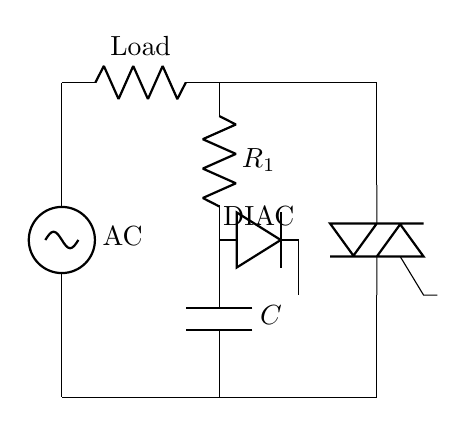
\begin{tikzpicture}
    \draw (0,4) to[sV, l=AC] (0,0);
    \draw (0,4) to[R, l=Load] (2,4) -- (4,4);
    \draw (4,4) to[triac] (4,0) -- (0,0);
    
    % Trigger
    \draw (2,4) to[R, l=$R_1$] (2,2) to[C, l=$C$] (2,0);
    \draw (2,2) to[D] (3,2) -- (3,1.3); \node at (2.5, 2.3) {DIAC};
\end{tikzpicture}
\captionof{figure}{DIAC-TRIAC Power Control}
\end{center}

\begin{center}
\begin{tabulary}{\linewidth}{|L|L|}
\hline \textbf{Component} & \textbf{Function} \\ \hline
$R_1-C$ & Variable time constant for phase delay \\
DIAC & Triggers TRIAC when capacitor voltage reaches breakover \\
TRIAC & Controls load current based on triggering point \\
Load & Receives partial AC waveform based on phase control \\
\hline
\end{tabulary}
\captionof{table}{Circuit Components}
\end{center}

\begin{itemize}
    \item \keyword{Phase control}: RC network creates delay in triggering point within AC cycle
    \item \keyword{Bidirectional operation}: Works on both halves of AC cycle
\end{itemize}
\end{solutionbox}
\mnemonicbox{Delay Initiates At Capacitor, Triggers Reliable Independent AC Control}

\questionmarks{4(c) OR}{7}{Explain IC555 three stage sequential timer working with waveform.}

\begin{solutionbox}
A three-stage sequential timer uses multiple 555 ICs to generate timed sequences for process control.

\begin{center}
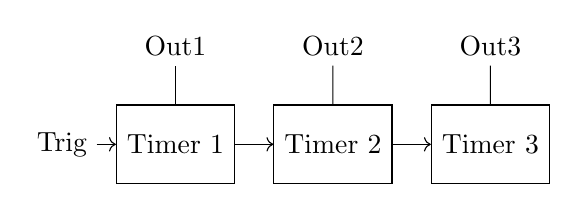
\begin{tikzpicture}[gtu block/.style={draw, rectangle, minimum width=1.5cm, minimum height=1cm}, node distance=2cm]
    \node[gtu block] (T1) {Timer 1};
    \node[gtu block, right of=T1] (T2) {Timer 2};
    \node[gtu block, right of=T2] (T3) {Timer 3};
    
    \draw[->] (-1,0) node[left]{Trig} -- (T1);
    \draw[->] (T1) -- (T2);
    \draw[->] (T2) -- (T3);
    
    \draw (T1) -- (0,1) node[above]{Out1};
    \draw (T2) -- (2,1) node[above]{Out2};
    \draw (T3) -- (4,1) node[above]{Out3};
\end{tikzpicture}
\captionof{figure}{Sequential Timer Logic}
\end{center}

\begin{center}
\begin{tabulary}{\linewidth}{|L|L|L|L|}
\hline \textbf{Stage} & \textbf{Action} & \textbf{Duration} & \textbf{Next Stage Trigger} \\ \hline
Initial & All outputs LOW & - & External trigger \\
Stage 1 & Output 1 HIGH & T1 ($R_1 C_1$) & Output 1 falling edge \\
Stage 2 & Output 2 HIGH & T2 ($R_2 C_2$) & Output 2 falling edge \\
Stage 3 & Output 3 HIGH & T3 ($R_3 C_3$) & Output 3 falling edge \\
Reset & All outputs LOW & T4 (reset time) & New external trigger \\
\hline
\end{tabulary}
\captionof{table}{Sequential Timing}
\end{center}

\begin{itemize}
    \item \keyword{Cascading connection}: Output of first timer triggers second, and so on
    \item \keyword{Timing control}: Each stage duration independently adjustable with RC values
\end{itemize}
\end{solutionbox}
\mnemonicbox{First Stage Finishes, Second Starts, Third Succeeds}

\questionmarks{5(a)}{3}{Draw and explain solid state control of DC shunt motor.}

\begin{solutionbox}
Solid-state DC motor control uses SCRs to regulate voltage applied to the motor.

\begin{center}
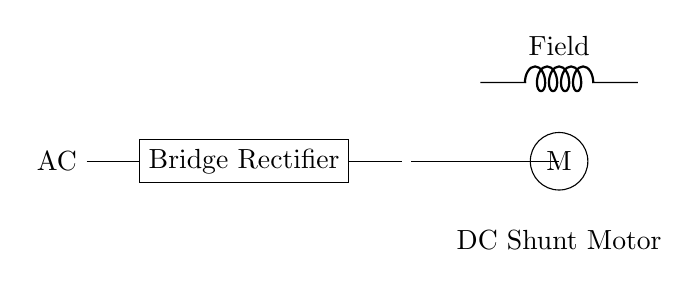
\begin{tikzpicture}
    % Bridge Rectifier feeding Motor
    \draw (0,0) node[draw, rectangle] (rect) {Bridge Rectifier};
    \draw (-2, 0) node[left]{AC} -- (rect);
    \draw (rect) -- (2,0) node[thyristor] (T) {};
    \draw (T.east) -- (4,0) node[draw, circle] (M) {M};
    \node at (4, -1) {DC Shunt Motor};
    
    % Field
    \draw (3, 1) to[L, l=Field] (5,1);
\end{tikzpicture}
\captionof{figure}{Solid State DC Motor Control}
\end{center}

\begin{center}
\begin{tabulary}{\linewidth}{|L|L|L|}
\hline \textbf{Method} & \textbf{Operation} & \textbf{Advantage} \\ \hline
Phase control & Varies SCR firing angle & Smooth speed control \\
Chopper control & Pulse width modulation & High efficiency \\
Closed-loop & Feedback from tachometer & Precise speed regulation \\
\hline
\end{tabulary}
\captionof{table}{Control Methods}
\end{center}

\begin{itemize}
    \item \keyword{Speed regulation}: Controls armature voltage to vary motor speed
    \item \keyword{Torque control}: Maintains high starting torque with current limiting
\end{itemize}
\end{solutionbox}
\mnemonicbox{SCR Controls Current Delivering Motor Power}

\questionmarks{5(b)}{4}{Explain working principle of stepper motor.}

\begin{solutionbox}
Stepper motors convert digital pulses into precise mechanical rotation through electromagnetic principles.

\begin{center}
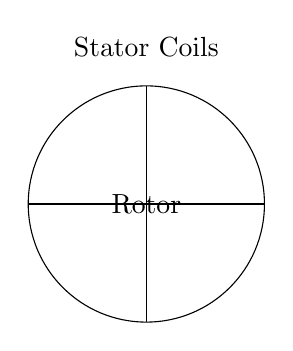
\begin{tikzpicture}
    \draw (0,0) circle (1.5);
    \foreach \a in {0, 90, 180, 270} \draw (0,0) -- (\a:1.5);
    \node at (0,0) {Rotor};
    \node at (0,2) {Stator Coils};
\end{tikzpicture}
\captionof{figure}{Stepper Motor Concept}
\end{center}

\begin{center}
\begin{tabulary}{\linewidth}{|L|L|L|}
\hline \textbf{Step Type} & \textbf{Rotation Angle} & \textbf{Control Method} \\ \hline
Full step & Typically $1.8^{\circ}$ or $0.9^{\circ}$ & One phase at a time \\
Half step & Half of full step & Two phases alternating \\
Micro-step & Fraction of full step & PWM current control \\
Wave drive & Full step angle & One phase energized \\
\hline
\end{tabulary}
\captionof{table}{Stepping Modes}
\end{center}

\begin{itemize}
    \item \keyword{Digital positioning}: Each pulse rotates motor by precise angle
    \item \keyword{Holding torque}: Maintains position when energized without rotation
\end{itemize}
\end{solutionbox}
\mnemonicbox{Pulses Produce Precise Positional Steps}

\questionmarks{5(c)}{7}{Draw the block diagram of PLC and explain function of each block.}

\begin{solutionbox}
Programmable Logic Controller (PLC) is an industrial digital computer for automation control.

\begin{center}
\begin{tikzpicture}[gtu block/.style={draw, rectangle, minimum width=2.5cm, minimum height=1.2cm}, node distance=3cm]
    \node[gtu block] (cpu) {CPU};
    \node[gtu block, left of=cpu] (in) {Input Module};
    \node[gtu block, right of=cpu] (out) {Output Module};
    \node[gtu block, below of=cpu] (mem) {Memory};
    \node[gtu block, above of=cpu] (pwr) {Power Supply};
    
    \draw[<->] (in) -- (cpu);
    \draw[<->] (cpu) -- (out);
    \draw[<->] (cpu) -- (mem);
    \draw[->] (pwr) -- (cpu);
\end{tikzpicture}
\captionof{figure}{PLC Architecture}
\end{center}

\begin{center}
\begin{tabulary}{\linewidth}{|L|L|}
\hline \textbf{Component} & \textbf{Function} \\ \hline
Power Supply & Converts main power to DC required by PLC \\
CPU & Executes program and makes decisions based on I/O \\
Memory & Stores program and data (ROM, RAM, EEPROM) \\
Input Module & Interfaces with sensors, switches, encoders \\
Output Module & Controls actuators, motors, valves, indicators \\
Communication Module & Connects to other PLCs, computers, networks \\
Programming Device & Used to write, edit, monitor PLC programs \\
\hline
\end{tabulary}
\captionof{table}{PLC Modules}
\end{center}

\begin{itemize}
    \item \keyword{Scan cycle}: Reads inputs, executes program, updates outputs continuously
    \item \keyword{Programming languages}: Ladder logic, function block, structured text, etc.
\end{itemize}
\end{solutionbox}
\mnemonicbox{Power Centralizes Processing, Inputs/Outputs Make Automation}

\questionmarks{5(a) OR}{3}{Draw and explain construction of DC Servo motor.}

\begin{solutionbox}
DC servo motors provide precise position control with feedback for automation and robotics.

\begin{center}
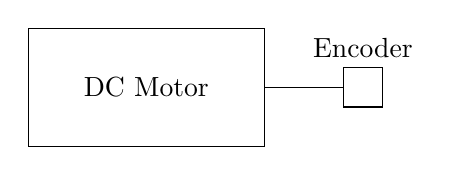
\begin{tikzpicture}
    \draw (0,0) rectangle (3,1.5);
    \node at (1.5, 0.75) {DC Motor};
    \draw (3, 0.75) -- (4, 0.75); % Shaft
    \draw (4, 0.5) rectangle (4.5, 1); % Encoder
    \node[above] at (4.25, 1) {Encoder};
\end{tikzpicture}
\captionof{figure}{DC Servo Motor}
\end{center}

\begin{center}
\begin{tabulary}{\linewidth}{|L|L|}
\hline \textbf{Component} & \textbf{Function} \\ \hline
Armature & Rotates within magnetic field \\
Field magnets & Creates magnetic field (often permanent magnets) \\
Commutator & Transfers power to rotating armature \\
Feedback device & Encoder/tachometer for position/speed feedback \\
Brushes & Connect power to commutator \\
\hline
\end{tabulary}
\captionof{table}{Servo Components}
\end{center}

\begin{itemize}
    \item \keyword{Low inertia}: Special design allows rapid acceleration/deceleration
    \item \keyword{High torque-to-inertia ratio}: Responds quickly to control signals
\end{itemize}
\end{solutionbox}
\mnemonicbox{Precise Position Feedback Drives Exact Control}

\questionmarks{5(b) OR}{4}{Explain working of BLDC motor.}

\begin{solutionbox}
Brushless DC (BLDC) motors use electronic commutation instead of mechanical brushes and commutator.

\begin{center}
\begin{tabulary}{\linewidth}{|L|L|}
\hline \textbf{Component} & \textbf{Function} \\ \hline
Stator & Fixed windings that generate rotating magnetic field \\
Rotor & Permanent magnets that follow rotating field \\
Electronic controller & Replaces mechanical commutation \\
Hall sensors & Detect rotor position for synchronized switching \\
Driver circuit & Provides sequence of currents to stator coils \\
\hline
\end{tabulary}
\captionof{table}{BLDC Components}
\end{center}

\begin{itemize}
    \item \keyword{Commutation}: Electronic switching sequences power to stator windings
    \item \keyword{Efficiency}: Higher efficiency due to elimination of brush losses
    \item \keyword{Reliability}: No brush wear or sparking, longer lifespan
\end{itemize}
\end{solutionbox}
\mnemonicbox{Electronic Switching Creates Rotation Without Brushes}

\questionmarks{5(c) OR}{7}{Explain construction and working of VFD.}

\begin{solutionbox}
Variable Frequency Drive (VFD) controls AC motor speed by varying frequency and voltage.

\begin{center}
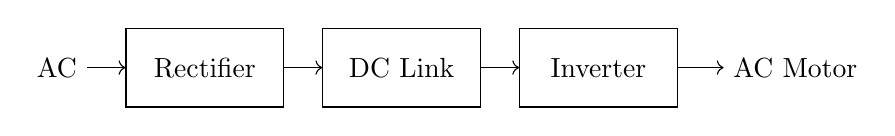
\begin{tikzpicture}[gtu block/.style={draw, rectangle, minimum width=2cm, minimum height=1cm, align=center}, node distance=2.5cm]
    \node[gtu block] (rect) {Rectifier};
    \node[gtu block, right of=rect] (dc) {DC Link};
    \node[gtu block, right of=dc] (inv) {Inverter};
    \node[right of=inv] (motor) {AC Motor};
    
    \draw[->] (-1.5,0) node[left]{AC} -- (rect);
    \draw[->] (rect) -- (dc);
    \draw[->] (dc) -- (inv);
    \draw[->] (inv) -- (motor);
\end{tikzpicture}
\captionof{figure}{VFD Block Diagram}
\end{center}

\begin{center}
\begin{tabulary}{\linewidth}{|L|L|L|}
\hline \textbf{Section} & \textbf{Components} & \textbf{Function} \\ \hline
Rectifier & Diodes/SCRs & Converts AC to DC \\
DC Bus & Capacitors, inductors & Filters and smooths DC \\
Inverter & IGBTs/transistors & Converts DC to variable frequency AC \\
Control circuit & Microprocessor & Controls switching frequency and patterns \\
Cooling system & Fans, heat sinks & Maintains safe operating temperature \\
Protection circuits & Sensors, relays & Prevents damage from faults \\
\hline
\end{tabulary}
\captionof{table}{VFD Structure}
\end{center}

\begin{itemize}
    \item \keyword{Speed control}: V/f ratio maintained to provide constant torque
    \item \keyword{Energy savings}: Adjusts power to actual load requirements
\end{itemize}
\end{solutionbox}
\mnemonicbox{Rectify, Filter, Invert Frequency For Motor Control}

\end{document}
